\documentclass[11pt]{amsart}
%prepared in AMSLaTeX, under LaTeX2e
\addtolength{\oddsidemargin}{-.55in} 
\addtolength{\evensidemargin}{-.55in}
\addtolength{\topmargin}{-.2in}
\addtolength{\textwidth}{1.0in}
\addtolength{\textheight}{.4in}

\renewcommand{\baselinestretch}{1.1}

\usepackage{verbatim,fancyvrb}

\usepackage{palatino,amssymb}

\usepackage{tikz}
\usetikzlibrary{arrows.meta}

\newtheorem*{thm}{Theorem 16.0}
\newtheorem*{defn}{Definition}
\newtheorem*{example}{Example}
\newtheorem*{problem}{Problem}
\newtheorem*{remark}{Remark}

\newcommand{\mtt}{\texttt}
\usepackage{alltt,xspace}
\newcommand{\mfile}[1]
{\medskip\begin{quote}\scriptsize \begin{alltt}\input{#1.m}\end{alltt} \normalsize\end{quote}\medskip}

%\usepackage[final]{graphicx}

\usepackage[pdftex, colorlinks=true, plainpages=false, linkcolor=blue, citecolor=red, urlcolor=blue]{hyperref}

% macros
\newcommand{\bc}{\mathbf{c}}
\newcommand{\br}{\mathbf{r}}
\newcommand{\bv}{\mathbf{v}}
\newcommand{\bx}{\mathbf{x}}
\newcommand{\by}{\mathbf{y}}

\newcommand{\CC}{\mathbb{C}}
\newcommand{\RR}{\mathbb{R}}
\newcommand{\ZZ}{\mathbb{Z}}

\newcommand{\eps}{\epsilon}
\newcommand{\grad}{\nabla}
\newcommand{\lam}{\lambda}
\newcommand{\lap}{\triangle}

\newcommand{\ip}[2]{\ensuremath{\left<#1,#2\right>}}

%\renewcommand{\det}{\operatorname{det}}
\newcommand{\onull}{\operatorname{null}}
\newcommand{\rank}{\operatorname{rank}}
\newcommand{\range}{\operatorname{range}}

\newcommand{\prob}[1]{\bigskip\noindent\textbf{#1.}\quad }
\newcommand{\exer}[2]{\prob{Exercise #2 in Lecture #1}}

\newcommand{\pts}[1]{(\emph{#1 pts}) }
\newcommand{\epart}[1]{\medskip\noindent\textbf{(#1)}\quad }
\newcommand{\ppart}[1]{\,\textbf{(#1)}\quad }

\newcommand{\Matlab}{\textsc{Matlab}\xspace}

\DefineVerbatimEnvironment{mVerb}{Verbatim}{numbersep=2mm,
frame=lines,framerule=0.1mm,framesep=2mm,xleftmargin=4mm,fontsize=\footnotesize}

\newcommand{\ema}{\emach}
\newcommand{\emach}{\eps_{\!_{\text{m}}}}


\begin{document}
\scriptsize \noindent Math 661 Optimization (Bueler) \hfill 23 August, 2016
\normalsize

\medskip\bigskip
\Large
\centerline{Five example optimization problems}

\bigskip\medskip
\normalsize

\thispagestyle{empty}

Starting this course with five examples makes sense.  The textbook\footnote{Nocedal \& Wright, \emph{Numerical Optimization}, 2nd ed., 2006} does not give any such fleshed-out examples, but all the experts have been exposed to many such examples.

There are three goals in starting this way:
\renewcommand{\labelenumi}{\arabic{enumi})}
\begin{enumerate}
\item To suggest how optimization can come from real-world applications.
\item To allow you to create, for yourself, some of the basic ideas theoretical and numerical ideas for how to solve such problems.
\item To provide examples on which to practice/learn \Matlab\footnote{Or Octave, which runs the same programs.  Or you can use other languages such as Python.} programming.
\end{enumerate}
On goal 2), your method \emph{may be ``brute force'' or inefficient \dots which is just fine!}

Assignment \#1 is based on these examples.  (Later Assignments will be largely based on textbook exercises, but I'll add my own problems and examples when needed.)  Note that each example has a ``code name'' like ``\texttt{calcone}'' which I will use to name my corresponding \Matlab code (``\texttt{calcone.m}'') when I hand out solutions to A \#1.

\bigskip
\renewcommand{\labelenumi}{\Roman{enumi}. \quad}
\begin{enumerate}
\item (\texttt{calcone})  \quad Let
    $$f(x) = \left(x^2 + \cos x\right)^2 - 10 \sin(5 x).$$
Compute
    $$\min_{x\in [0,2]} f(x)$$

You may write the same problem as an inequality-constrained optimization in form (1.1), on page 3 of the textbook, namely as
	$$\min_{x\in\RR} f(x) \qquad \text{subject to }\quad \begin{matrix} x \ge 0 \\ 2 - x \ge 0\end{matrix}$$
In this standard form, $\mathcal{E}=\emptyset$, $\mathcal{I}=\{1,2\}$, $c_1(x)=x$, and $c_2(x)=2-x$.  However, I assert no particular benefit to this standardized form in this case.

You saw such problems in Calculus I.  This one is hard to do by hand; it benefits from some programming and visualization using \Matlab.  Start your solution by plotting $f(x)$ on the given interval; you'll know something close to the solution just from that picture.


\medskip
\item (\texttt{fit})  \quad Consider the following 11 data which are plotted below:

\bigskip
\begin{tabular}{c|ccccccccccc}
x & 0.000 & 0.100 & 0.200 & 0.300 & 0.400 & 0.500 & 0.600 & 0.700 &  0.800 &  0.900 &  1.000 \\
\hline
y & 4.914 & 3.666 & 2.289 & 1.655 & 1.029 & 0.739 & 0.393 & 0.090 & -0.197 & -0.721 & -0.971
\end{tabular}

\bigskip
\begin{center}
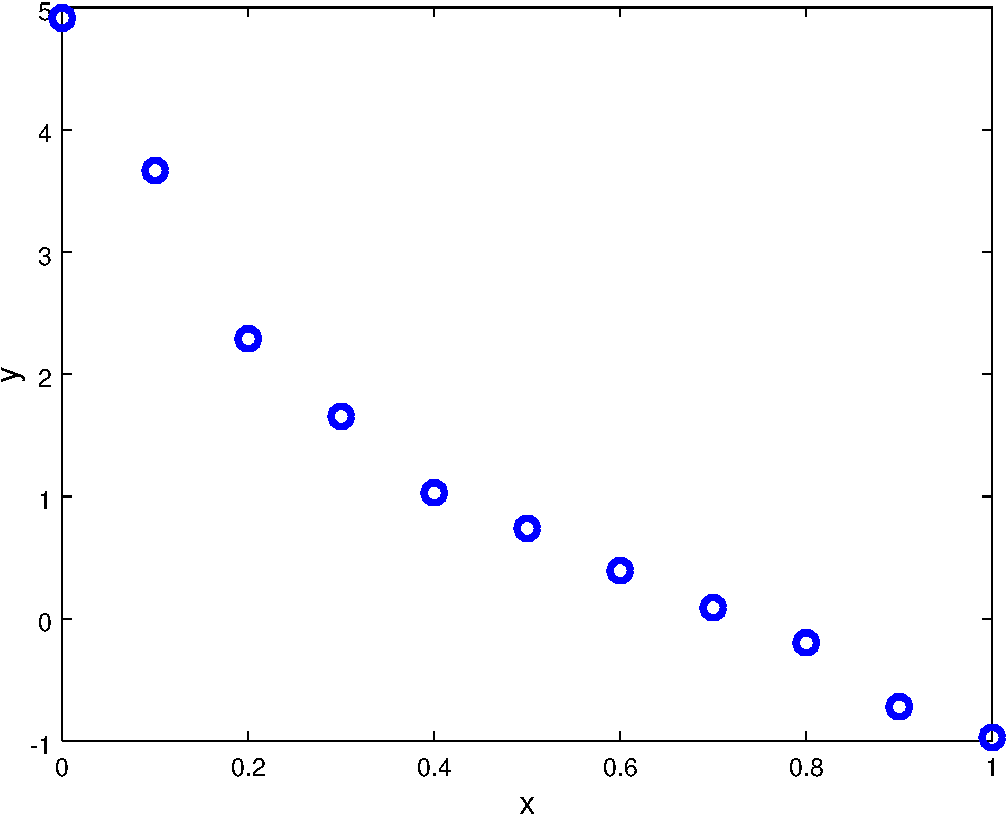
\includegraphics[width=0.6\textwidth]{fitdata}
\end{center}

\medskip
Suppose we believe that this data can be fit by a function of the form
	$$g(x) = c_1 + c_2 x + c_3 e^{-5 x}.$$
If the sense of ``fit'' is that the sum of the squares of the misfits should be as small as possible then we would solve
	$$\min_{c \in \RR^3} f(c)$$
where we define the objective function to be
	$$f(c) = \frac{1}{2} \sum_{j=1}^{11} \left(g(x_j) - y_j\right)^2 = \frac{1}{2} \sum_{j=1}^{11} \left(c_1 + c_2 x_j + c_3 e^{-5 x_j} - y_j\right)^2.$$

This problem is already in form (1.1) from the textbook, with $c = \left[c_1,c_2,c_3\right]$ an unknown vector of coefficients in $\RR^3$, and with no constraints ($\mathcal{E}=\emptyset,\mathcal{I}=\emptyset$).  Here $x_j,y_j$ are the data, with $x_j = 0.1 (j-1)$ regularly-spaced.  Note we are \emph{not} finding $x_j$ or $y_j$ values in the minimization process; these values merely determine the objective function.  Also note that the overall factor of $1/2$ in defining the function $f(\bc)$ is just a convenience for differentiating.\footnote{\dots a hint about the standard algorithms for finding the minimum.}

\medskip
\item (\texttt{salmon})  \quad Ed and Thomas caught 21 salmon, and all will be filleted.  Of these, $x_1$ will be eaten fresh, which requires 2 time units per fish.  Also, $x_2$ will be vacuum-packed and frozen (3 time units per fish) and another $x_3$ will be smoked, vacuum-packed, and frozen (4 time units per fish).  Thus the total amount of processing time is $2 x_1 + 3 x_2 + 4 x_3$.  However, at most 2 fish can be eaten fresh before they go bad, and at most 10 fish can be smoked in the time allowed.

Finding $x_1,x_2,x_3$ to minimize the total processing time means solving this constrained problem with $f(x) = 2 x_1 + 3 x_2 + 4 x_3$:
	$$\min_{x\in\RR^3} f(x) \qquad \text{subject to }\quad \begin{matrix} x_1 + x_2 + x_3 = 21 \\ 0 \le x_1 \le 2 \\ 0 \le x_2 \\ 0 \le x_3 \le 10 \end{matrix}$$

This problem is not quite in standard form (1.1) because the inequality constraints are not all in the form ``$c_i(x) \ge 0$.''  An easy exercise on Assignment \#1 asks you to put it in standard form.

\medskip
\item (\texttt{tsp})  \quad Jill sells amazing devices which make your brain absorb math more easily.  To sell these devices she plans to visit cities A, F, J, N, W starting and ending at city S.  Some pairs of cities have connecting flights and some do not; the one-way costs of the various flights are shown below in a \emph{graph} with costs (``weights'') on each connection (``edge'').  It is clear to Jill that she should visit each city exactly once, except for returning to S at the end, so a possible itinerary is expressible as a seven letter string like ``SANFWJS.''

\begin{tikzpicture}[scale=0.9]
\begin{scope}[every node/.style={circle,thick,draw}]
    \node (A) at (-0.5,0) {A};
    \node (F) at (0,3)    {F};
    \node (J) at (2,-1)   {J};
    \node (N) at (-3,3)   {N};
    \node (S) at (3,-3)   {S};
    \node (W) at (3,1)    {W} ;
\end{scope}

\begin{scope}[every node/.style={fill=white},
              every edge/.style={draw=black,very thick}]
    \path (A) edge node {$100$} (F);
    \path (A) edge node {$100$} (J);
    \path (A) edge node {$150$} (N);
    \path (A) edge[bend right=50] node {$250$} (S);
    \path (A) edge node {$150$} (W);
    %\path (F) edge node {$150$} (J);
    \draw[very thick] (F.east) .. controls (3,4) and (6,0) .. (J.east) node[midway] {$150$};
    \path (F) edge node {$200$} (N);
    %\path (F) edge node {$300$} (S);
    \draw[very thick] ([yshift=3mm,xshift=-1mm] F.east) .. controls (4,5) and (7,-1) .. (S.east) node[midway] {$300$};
    \path (F) edge node {$250$} (W);
    \path (J) edge node {$200$} (S);
    \path (J) edge node {$200$} (W);
\end{scope}
\end{tikzpicture}

This is an example of the famous \emph{traveling salesperson problem}.  If $x$ denotes a seven-letter sting containing valid connecting flights, an itinerary, then we may define the objective function $f(x)$ to be the cost of that itinerary.  Thus $f(x)$ is defined using the edge weights below.  Note that finding even one valid (``feasible'') itinerary may already be nontrivial, at for more complicated graphs.

The problem \emph{could} be written
	$$\min_{x \text{ is valid itinerary}} f(x)$$
but this does \emph{not} mean it is in standard form (1.1).  There is no sensible way to treat the possible inputs $x$ as ``$x \in \RR^n$,'' even with constraints, as written in (1.1).  That is, the traveling salesperson problem is a \emph{discrete optimization} problem, not a continuous optimization problem.

\medskip
\item (\texttt{beam})  \quad 
\end{enumerate}

\end{document}

